\begin{table}[!htbp]
\centering
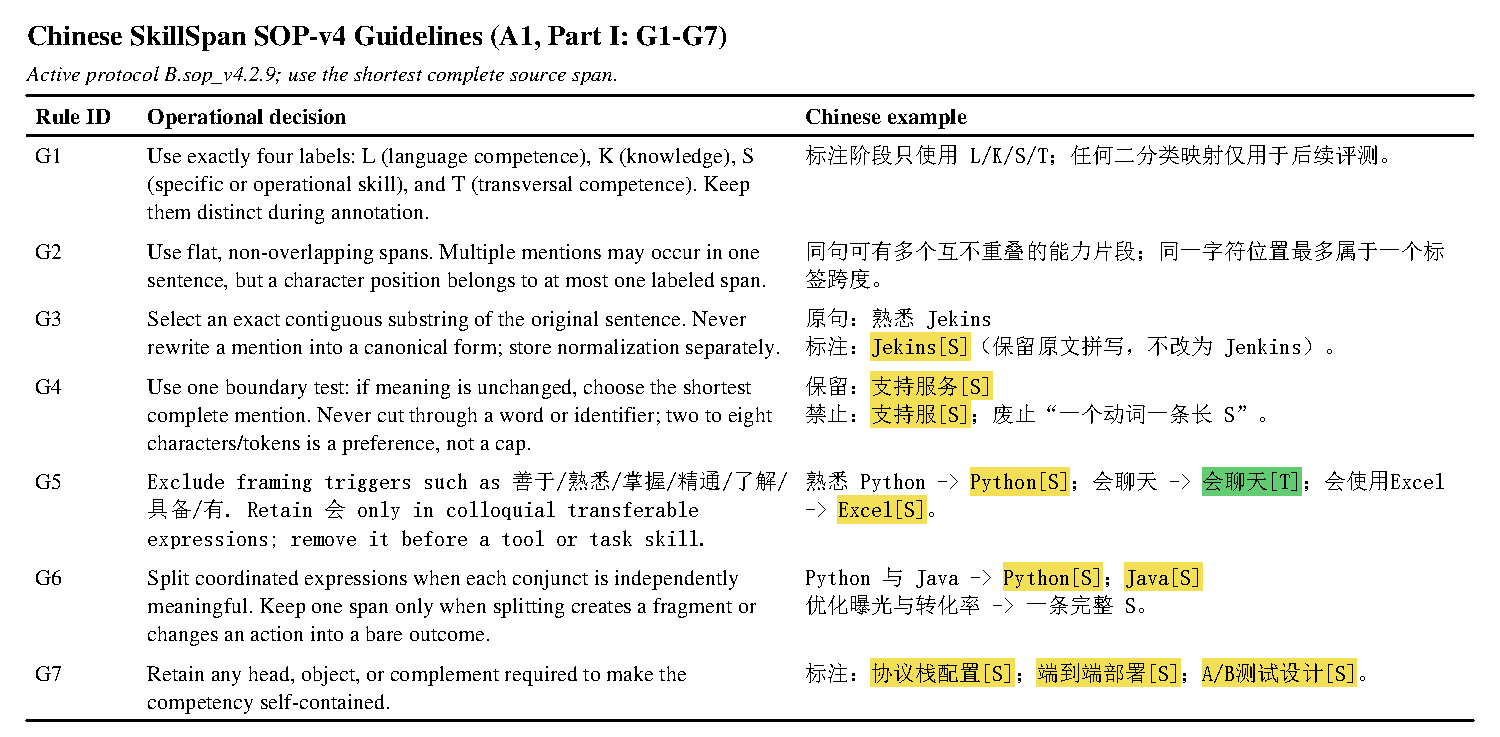
\includegraphics[width=\linewidth,keepaspectratio]{image/appendix_annotation_tables/A1a_Chinese_Skillspan_General_Annotation_Guidelines_Part_1.pdf}
\caption{Standardized \texttt{B.sop\_v4.2.9} guidelines, Part I (G1--G7). The panel defines exact source substrings, meaning-preserving shortest-complete boundaries, contextual trigger handling, coordination splitting, and necessary complements.}
\label{tab:annotation-general-a}
\end{table}
